Ein Codierungsverfahren verwendet die Zeichen
$\Sigma=\{
\clubsuit,
\diamondsuit,
\spadesuit,
\heartsuit
\}$.
Aus technischen Gründen wird verlangt, dass die Anzahlen der 
verschiedenen Zeichen in einem Wort sich möglichst nicht unterscheiden, was
exakt natürlich nur möglich ist, wenn die Wortlänge durch vier
teilbar ist.
Für zwei beliebige Zeichen $a,b\in\Sigma$ wird gefordert, dass
\[
|\, |w|_a - |w|_b\,|\le 1,
\]
die Anzahlen der Zeichen in einem Wort unterscheiden sich also höchstens
um $1$.
Bei binärer Codierung ist diese Eigenschaft
als {\em DC-balance} bekannt.
Im binären Fall lässt sich DC-balance leicht mit einem Stackautomaten
prüfen.
Ist dies in diesem Fall mit vier Zeichen auch möglich?

\themaL{Pumping Lemma fur kontextfreie Sprachen}{Pumping Lemma für kontextfreie Sprachen}
\thema{Grammatik}

\begin{loesung}
Es geht darum, ob die Sprache
\[
L
=
\{w\in\Sigma^*\,|\;
|\, |w|_a - |w|_b\,|\le 1\;\forall a,b\in\Sigma(a\ne b)\}
\]
kontextfrei ist.
$L$ ist aber nicht kontextfrei, wie wir mit dem Pumping-Lemma für
kontextfreie Sprachen nachweisen können:
\begin{enumerate}
\item 
Wir nehmen an, dass $L$ kontextfrei ist.
\item
Nach dem Pumping-Lemma für kontextfreie Sprachen gibt es eine Zahl
$N$ derart, dass Wörter $w\in L$ mit $|w|\ge N$ gepumpt werden.
\item
Wir konstruieren das Wort
\[
w = 
\clubsuit^N
\diamondsuit^N
\spadesuit^N
\heartsuit^N
 \in
L.
\]
\item
Nach dem Pumping Lemma für kontextfreie Sprachen lässt sich das Wort $w$
in fünf $w=uvxyz$ aufteilen derart, dass $|vxy|\le N$.
Eine möglich Aufteilung ist
\begin{center}
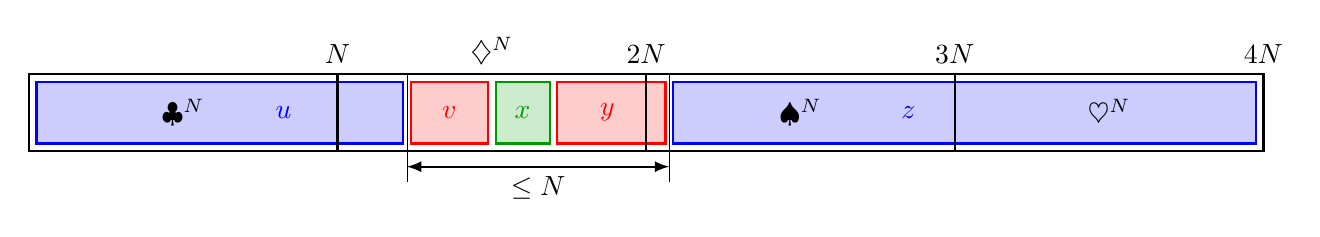
\begin{tikzpicture}[>=latex,thick,scale=0.98]
\definecolor{darkgreen}{rgb}{0,0.6,0}
\draw (0,0) rectangle (16,1);
\node at (4,1) [above] {$N$};
\node at (8,1) [above] {$2N$};
\node at (12,1) [above] {$3N$};
\node at (16,1) [above] {$4N$};
\fill[color=blue!20] (0.1,0.1) rectangle (4.85,0.9);
\draw[color=blue] (0.1,0.1) rectangle (4.85,0.9);
\fill[color=red!20] (4.95,0.1) rectangle (5.95,0.9);
\draw[color=red] (4.95,0.1) rectangle (5.95,0.9);
\fill[color=darkgreen!20] (6.05,0.1) rectangle (6.75,0.9);
\draw[color=darkgreen] (6.05,0.1) rectangle (6.75,0.9);
\fill[color=red!20] (6.85,0.1) rectangle (8.25,0.9);
\draw[color=red] (6.85,0.1) rectangle (8.25,0.9);
\fill[color=blue!20] (8.35,0.1) rectangle (15.9,0.9);
\draw[color=blue] (8.35,0.1) rectangle (15.9,0.9);
\draw (4,0)--(4,1);
\draw (8,0)--(8,1);
\draw (12,0)--(12,1);
\draw[line width=0.1pt] (4.9,1)--(4.9,-0.4);
\draw[line width=0.1pt] (8.3,1)--(8.3,-0.4);
\draw[<->] (4.9,-0.2)--(8.3,-0.2);
\node at (6.6,-0.2) [below] {$\le N$};
\node at (2,0.5) {$\clubsuit^N$};
\node at (6,1) [above] {$\diamondsuit^N$};
\node at (10,0.5) {$\spadesuit^N$};
\node at (14,0.5) {$\heartsuit^N$};
\node[color=blue] at (3.3,0.5) {$u$};
\node[color=red] at (5.45,0.5) {$v$};
\node[color=darkgreen] at (6.4,0.5) {$x$};
\node[color=red] at (7.5,0.5) {$y$};
\node[color=blue] at (11.4,0.5) {$z$};
\end{tikzpicture}
\end{center}
Der Block $vxy$ kann jedoch an jeder beliebigen Stelle innerhalb des
Wortes stehen.
\item
Die Teile $v$ und $y$ können höchstens zwei Arten von Zeichen im Wort $w$
enthalten, beim Pumpen ändert sich also maximal die Anzahl dieser
Zeichen.
Mindestens zwei Arten von Zeichen werden ihre Anzahl also beim Pumpen
nicht ändern.
Pumpt man mehr als einmal, wird der Unterschied der Anzahl der Zeichen,
die in $v$ und $y$ enthalten sind, um mehr als $1$ verändern und damit
um mehr, als gemäss Definition von $L$ tolerierbar ist.
Mehr als einmal Pumpen erzeugt also ein Wort, welches nicht mehr in
$L$ ist.
\item
Dieser Widerspruch zeigt, dass die Annahme im ersten Schritt nicht
zutreffen kann, dass also $L$ nicht kontextfrei sein kann.
\qedhere
\end{enumerate}
\end{loesung}

\begin{bewertung}
Annahme, dass die Sprache regulär ist ({\bf L}) 1 Punkt,
Pumping Length ({\bf N}) 1 Punkt,
Beispielwort ({\bf W}) 1 Punkt,
Aufteilung ({\bf A}) 1 Punkt,
Widerspruch beim Pumpen ({\bf P}) 1 Punkt,
Schlussfolgerung ({\bf S}) 1 Punkt.
Im 5.~Schritt ist wichtig darauf hinzuweisen,
dass mehr als einmal gepumpt werden muss, um den Widerspruch zu erzwingen.
\end{bewertung}


